%  article.tex (Version 3.3, released 19 January 2008)
%  Article to demonstrate format for SPIE Proceedings
%  Special instructions are included in this file after the
%  symbol %>>>>
%  Numerous commands are commented out, but included to show how
%  to effect various options, e.g., to print page numbers, etc.
%  This LaTeX source file is composed for LaTeX2e.

%  The following commands have been added in the SPIE class 
%  file (spie.cls) and will not be understood in other classes:
%  \supit{}, \authorinfo{}, \skiplinehalf, \keywords{}
%  The bibliography style file is called spiebib.bst, 
%  which replaces the standard style unstr.bst.  

\documentclass[]{spie}  %>>> use for US letter paper
%%\documentclass[a4paper]{spie}  %>>> use this instead for A4 paper
%%\documentclass[nocompress]{spie}  %>>> to avoid compression of citations
%% \addtolength{\voffset}{9mm}   %>>> moves text field down
%% \renewcommand{\baselinestretch}{1.65}   %>>> 1.65 for double spacing, 1.25 for 1.5 spacing 
%  The following command loads a graphics package to include images 
%  in the document. It may be necessary to specify a DVI driver option,
%  e.g., [dvips], but that may be inappropriate for some LaTeX 
%  installations. 
\usepackage[]{graphicx}
\usepackage{epstopdf}
\usepackage{url}
\usepackage{amsmath}
\title{Unveiling ALMA software behavior using a decoupled log analysis framework}

%>>>> The author is responsible for formatting the 
%  author list and their institutions.  Use  \skiplinehalf 
%  to separate author list from addresses and between each address.
%  The correspondence between each author and his/her address
%  can be indicated with a superscript in italics, 
%  which is easily obtained with \supit{}.

\author{Juan Pablo Gil$\supit{a}^{*}$, Alexis Tejeda\supit{b}, Tzu-Chiang Shen\supit{a}, Norman S\'aez\supit{a}
\skiplinehalf
\supit{a}Atacama Large Millimeter/submillimeter Array, Av. Alonso de C\'ordova 3107, Santiago, Chile\\
\supit{b}National Radio Astronomy Observatory (NRAO), Socorro, New Mexico, USA\\ $*$jgil@alma.cl
%\supit{b}Affiliation2, Address, City, Country
}

%>>>> Further information about the authors, other than their 
%  institution and addresses, should be included as a footnote, 
%  which is facilitated by the \authorinfo{} command.

\authorinfo{Further author information: Juan Pablo Gil: E-mail: jgil@alma.cl}
%%>>>> when using amstex, you need to use @@ instead of @
 

%%%%%%%%%%%%%%%%%%%%%%%%%%%%%%%%%%%%%%%%%%%%%%%%%%%%%%%%%%%%% 
%>>>> uncomment following for page numbers
% \pagestyle{plain}    
%>>>> uncomment following to start page numbering at 301 
%\setcounter{page}{301} 
 
  \begin{document} 
  \maketitle 

%%%%%%%%%%%%%%%%%%%%%%%%%%%%%%%%%%%%%%%%%%%%%%%%%%%%%%%%%%%%% 
\begin{abstract}
ALMA Software is a complex distributed system installed in more than one
hundred of computers, which interacts with more than one thousand of hardware
device components. A normal observation follows a flow that interacts with
almost that entire infrastructure in a coordinated way. The Software Operation
Support team (SOFTOPS) comprises specialized engineers, which analyze the generated
software log messages in daily basis to detect bugs, failures and predict
eventual failures. These log message can reach up to 30 GB per day. We describe
a decoupled and non-intrusive log analysis framework and implemented tools to
identify well known problems, measure times taken by specific tasks and detect
abnormal behaviors in the system in order to alert the engineers to take
corrective actions. The main advantage of this approach among others is that
the analysis itself does not interfere with the performance of the production
system, allowing to run multiple analyzers in parallel. In this paper we'll
describe the selected framework and show the result of some of the implemented
tools.
\end{abstract}

%>>>> Include a list of keywords after the abstract 

\keywords{bug, detection, log, analyzer}

%%%%%%%%%%%%%%%%%%%%%%%%%%%%%%%%%%%%%%%%%%%%%%%%%%%%%%%%%%%%%
\section{INTRODUCTION}\label{sec:intro}  % \label{} allows reference to this section
The Atacama Large Millimeter/sub-millimeter Array (ALMA) is currently the
world's largest astronomical facility, built in partnership with Europe,
    North America and East Asia in cooperation with the Republic of Chile. Its
    frequency coverage has a range from the mm/submm windows up to 1 THz. The
    observatory is placed in Atacama Desert at an altitude of 5000 meters above
    sea level, and it is controlled from the operations support facility at
    2.900 meters.

The software that controls the overall operations of the array, data processing
and later storage is based on top of ALMA Common Software (ACS), which runs in
a highly distributed environment including hardware and computers. The logs
generated by the different components of software contains valuable information
such data rates, uncommon behaviour of hardware, times involved in the
different stages of observations, etc. However, due to the high amount of those
logs most of that information remains hidden and are useless in practical terms,
except for a small set which is used to do daily troubleshooting activities.

A dedicated team of engineers, SOFTOPS, provides frontline
software support for the ALMA software among other activities\cite{gonzalez2010first}.
The usual workflow is to receive problem reports and determine the root cause of
the failures. This task is done by manually analyzing the logs around the time of
the event, and sometimes developing tools to extract specific information from
the whole set of logs in order to diagnose one specific problem. This approach
works well as reactive measures to solve problems, but don´t makes full usage
of most of the information inside the logs. Also, the time spent in find the
right logs among hundred or thousands of lines can be in the order of hours.

In this paper we describe generalities of ALMA software and its log system, and
describe a tool under development to make better usage of the information
already being stored in the logs through automated tools that do not interfere
with the normal operation of the array.

\section{ALMA Software and Logging Service}
ALMA Common Software (ACS) is the framework used in the logical infrastructure
for ALMA operation. ACS is based on CORBA and provides low level services,
    network abstraction and common design patterns for distributed software,
    based in a component / container paradigm\cite{schwarz2004alma}.

ACS deploys one dedicated notify service for the logging system that gets
distributed over the network in a publisher-subscriber paradigm and is used
intensively in each component. The logging service receives log entries from
all the system and distributes them to registered clients in a centralized
way. Each log has an associated priority and timestamp, allowing filtering at
different levels of the system. The logs consumers (clients) can access log
entries by subscribing to the event channel of interest.

A log is represented as a XML document that contains: a timestamp encoded in
ISO 8601 with precision up to millisecond; some fields of source code
information like file, line and/or routine; runtime context information
including host name, thread; the priority of the log that covers from Trace (1)
to Emergency (11); and the log message itself that is stored as CDATA\cite{avarias2010introducing}.
 
In ALMA production environment a dedicated set of hardware are used to run ACS
and all the software components. There are a number of clients normally running
during observation. The standard client used for the operators of the array is
jLog, a JAVA application that subscribes to logging channel and shows it in a
GUI with some basic tools to filter and search by different criteria. Another
client redirects logs to a relational database, and also stores them in XML
files in one of the servers in a FIFO scheme, typically keeping it at most two
days due to space restrictions\cite{shen2012alma}.

\section{Decoupled Log Infrastructure}
Although the log information is available both in XML files and in the
database, they are confined in the same environment and hardware used in
operation. Thus the analysis cannot be performed inside those machines to not
interfere with resources that must be fully dedicated to operate the array. For
that reason, we developed a client that acts as a proxy between the centralized
ALMA logging system and an external infrastructure including a database and a
dedicated machine to perform log analysis. The idea behind this design is to
protect as much as possible the logging channel of ALMASW to not saturate the
connection to that channel, instead, connecting to the external queue

%-------------
   \begin{figure}[!ht]
   \begin{center}
   \begin{tabular}{c}
   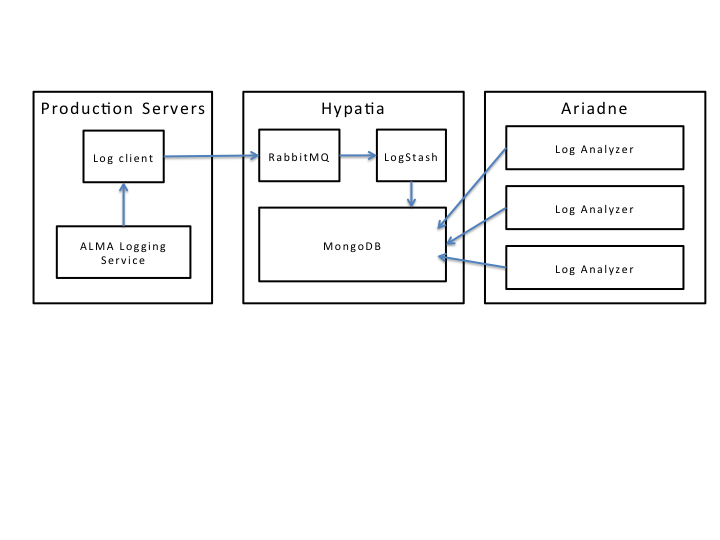
\includegraphics[height=8.0cm]{../img/image1-decoupled.png}
   \end{tabular}
   \end{center}
   \caption[dc] 
   { \label{fig:dc} Decoupled log infrastructure}
   \end{figure} 
%-------------


The general infrastructure consists in 1) a new client that consumes logs and
send them to 2) a queue system using RabbitMQ\cite{RabbitMQ}, a log parser through 
LogStash\cite{LogStash} that sends the data in JSON inside MongoDB\cite{mongo}, and 3) a pool of clients that
analyses the logs through queries to MongoDB. Two servers were deployed for
this purpose, decoupled from production machines: Hypatia, who contains
RabbitMQ, LogStash and MongoDB, and Ariadne that works only to run the clients
and test different ideas.

\section{Log Client}
In order to deploy the log client it was used the source code of jLog,
   inheriting only the JAVA classes to work with Notification Channel
   subscription and some internal logic to buffer log messages to avoid the
   slow consumer problem\cite{mora2012alma}. To this barebones it was
   added the logic to send messages to RabbitMQ. In order to secure even more
   the protection of the logging channel, an extra buffer protection was
   developed, a internal memory buffer limited by the quantity of messages in
   the queue to be sent to RabbitMQ nor also limited by the amount of memory
   consumed by the queue, in which if the limit is raised, the application will
   delete all messages stored in the queue.

The log client is a work still under development, as ALMA is in production
state, any addition and software change must be carefully profiled and tested
to certify that there is no significant impact in overall performance. Initial
tests shows that both CPU usage and memory consumption are under control and
many Gb of logs have been already transferred to MongoDB without noticeable
impact on production servers.

\section{Queue and Database}
The log client running inside the observatory production servers uses RabbitMQ
as message broker. Next in the chain is LogStash\cite{LogStash} whose purpose is to
convert the XML string representing a log event to JSON to be ingested by
MongoDB. Also, LogStash add some new fields to the log instance:

1)  Origin. Besides production servers that controls the main array of antennas
(which is called ``AOS''), we have many small replicas with different
purposes like testing, commissioning, backup, etc. This field is used to
differentiate between sources, and also to store logs in separate collections
inside MongoDB. In AMQP terms\cite{AMQP}, the field origin act as routing key.  2)
Date. ALMA Log message has a timestamp associated using the format
{\tt 2014-05-25T00:12:59.021 }. But searching strings over millions of logs
is inefficient, so we also store the number of milliseconds elapsed since Unix
Epoch (Jan 1, 1970).

For each origin there is a separate collection. Also, to control the size of
the database the collections are capped, that is, they acts as a FIFO queue if
the size of the database exceeds some limit. In our initial testing we
specified the max size parameter in 100 Gb for AOS and 10 Gb for other
collections. For AOS it is expected to cover three days of normal operation
what is enough for the current analyzers that we have aready running.

Our initial database choice was ElasticSearch due its straighforward
integration with LogStash and the power of Kibana as a graphical interface to
do queries. ElasticSearch is a non-relational database, distributed and
scalable based on Lucene\cite{es}. But there were two reasons to switch to MongoDB:
ElasticSearch is oriented to faceted search that querying by applying multiple
filters and bringing results based on scores; and second, there are other
efforts inside ALMA that already uses MongoDB\cite{shenexploring}, then for
synergy and standardization MongoDB was the chosen one. Initially we deployed
MongoDB in a 32 bit machine but soon we found that it was not a smart choice.
The logs has a natural timing nature, and in order to use dates in an efficient
way MongoDB stores Date object using a  64 bit  representation.

\section{Log Analyzers}
One common task of the software team is to diagnose the cause of errors
reported by array operators. Some of them are repeated errors but in the
process to identify them as duplicated hours can be spent. As a practical
application and to overcome that problem it was developed an error detector
script using the infrastructure described above, given that its series of logs
are known and identify it uniquely. The main idea is search in MongoDB an
ordered sequence of event that if happens, then a specific error can be
classified as detected.

A broad class of errors happens at some point inside one observation. An
observation is a well defined process, which consists basically in the
initialization of resources, a serie of calibrations and actual sky
observations and finally storing the results in the database. Every observation
is performed in the context of one logical set of hardware resources called
Array, and there can be many arrays running observations simultaneously. 

Then, our problem is reduced to detect a sequence of logs that could appears
during one observation inside the lifecycle of an array, that can be many in
parallel. We choose to work with deterministic finite state machines, or
briefly finite state machines (FSM) because its simplicity and flexibility. A
FSM is completey defined by:

\begin{align*}
FSM &= (X,S,F,x_{0},g) \mbox{ where}\\
X & \mbox{ is a finite non-empty set of states}\\
S & \mbox{ is a finite set of input symbols}\\
F \subset X & \mbox{ are the final states}\\
x_{0} \in X & \mbox{ is the initial state}\\
g: X \times S \to X & \mbox{ is the transition function}
\end{align*}

A sequence of logs that describes an error can be transformed in a FSM if we
choose the input symbols S as the set of those logs, and the transition
function g traversing different states describing the ordered steps of expected
logs until the last one, ending in a ErrorDetected state. 

Due to the observation and array concepts described above, we also need to take
care about the lifecycles of the arrays and observations. So, any error
detector described by an FSM should include at least the array initialization
and array destructions states. The observation lifecycle is an analogous work,
    so we will focus only in the array lifecycle.

To implement the train of input symbols logic (or specific logs that represent
        them), a script using Python and Pymongo (a python client for mongoDB)
    was developed that creates a new FSM for each found array, searchs for each
    possible log given the current state, ordered by time, and considering only
    the first element if any. If it exists, the FSM changes its state
    accordingly and a new query is done until the last log is reached. If there
    are no more logs the script waits for incoming logs and repeats the process
    until a final state is reached.

%-------------
   \begin{figure}[!ht]
   \begin{center}
   \begin{tabular}{c}
   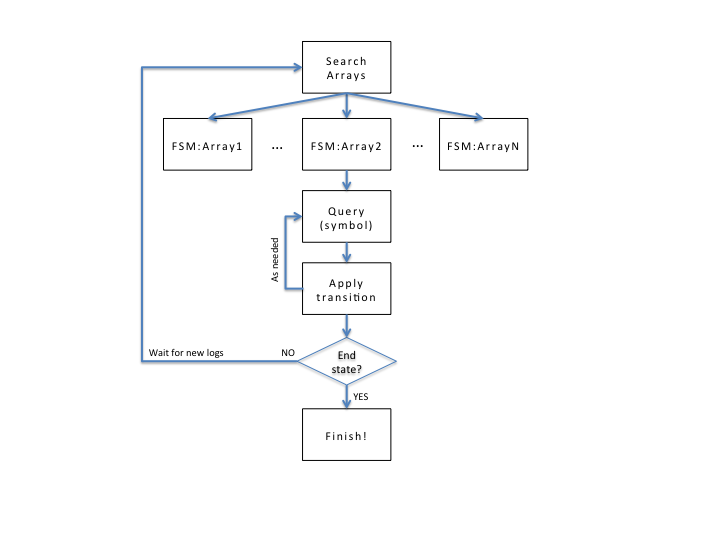
\includegraphics[height=8.0cm]{../img/FSM-flow-diagram.png}
   \end{tabular}
   \end{center}
   \caption[fsm] 
   { \label{fig:fsm} general state machine}
   \end{figure} 
%-------------

This script runs in Ariadne and querys Hypatia where MongoDB is deployed. The
program were done general: It reads the FSM specification from an external JSON
file. For example, the lifecycle array detector consists in this FSM
specification:
\begin{verbatim}
{
  "StartState" : "InitArray",
  "FinalStates" : [ "CommitSuicide" ],
  "States": {
    "InitArray" : 
      [
        { 
          "query": {
              "logMessage": {"$regex": "successfully released a component with curl=this.arrayName$"},
              "sourceObject": "CONTROL/ACC/javaContainer"
              },
          "nextState" : "CommitSuicide"
        }
      ],
    "CommitSuicide" : []
  }
}

\end{verbatim}

And the output in a given set of logs (near 3 millions representing near 2 hours of real operation) is as follow:
\begin{verbatim}
client-190-91-87-26:mongo joao$ ./testArray.py checkArrays.json
Using finite state machine: checkArrays.json
- New machine! CONTROL/Array001
- New machine! CONTROL/Array002
- New machine! CONTROL/Array003
--- CONTROL/Array001: "2014-03-21T20:31:32.534+00:00" client 'CONTROL/MASTER' has successfully 
released a component with curl=CONTROL/Array001
--- CONTROL/Array001: InitArray -> CommitSuicide
- Killing machine=CONTROL/Array001 because is in state CommitSuicide
- New machine! CONTROL/Array004
- New machine! CONTROL/Array005
--- CONTROL/Array002: "2014-03-21T20:40:33.051+00:00" client 'CONTROL/MASTER' has successfully 
released a component with curl=CONTROL/Array002
--- CONTROL/Array002: InitArray -> CommitSuicide
- Killing machine=CONTROL/Array002 because is in state CommitSuicide
- New machine! CONTROL/Array006
- New machine! CONTROL/Array007
--- CONTROL/Array004: "2014-03-21T20:50:30.522+00:00" client 'CONTROL/MASTER' has successfully 
released a component with curl=CONTROL/Array004
--- CONTROL/Array004: InitArray -> CommitSuicide
- Killing machine=CONTROL/Array004 because is in state CommitSuicide
--- CONTROL/Array006: "2014-03-21T21:39:46.518+00:00" client 'CONTROL/MASTER' has successfully 
released a component with curl=CONTROL/Array006
--- CONTROL/Array006: InitArray -> CommitSuicide
- Killing machine=CONTROL/Array006 because is in state CommitSuicide
It seems there is no more logs. Waiting 10 seconds until the new search.
It seems there is no more logs. Waiting 10 seconds until the new search.
It seems there is no more logs. Waiting 10 seconds until the new search.
Search disabled. Too much inactivity.
- Killing CONTROL/Array007 (InitArray) because I finished my searching and I will end.
- Killing CONTROL/Array005 (InitArray) because I finished my searching and I will end.
- Killing CONTROL/Array003 (InitArray) because I finished my searching and I will end.
\end{verbatim}

Extending this general behaviour is easy, but in order to see the real
performance of the system the log client that runs inside the production
servers must be installed and running continuously.

\section{Conclusions and Future Works}
It was showed in this work that heavy analysis can be done offline by using a
decoupled log database without interfere with normal operation of the
observatory. This was done by deploying well known tools and some theoretical
concepts like finite state machine which can be extended to many other expected
behaviours or known errors. 

A number of direct improvements are possible in the infrastructure described
above. The logging client must be deeply tested so it became part of the
software, subject to formal maintenance by ALMA engineers. Many more FSM should
be deployed to effectively show the usefulness of the infrastructure in daily
support work. To help the scientist and operators, it could be developed GUIs
and web pages the display early alerts of failures. In the theoretical side,
    the various finite state machines can be automatically merged in a bigger
    one that reuses the input symbols shared between them (i.e. far less
            queries to DB). 

As always, there are barriers for any new set of tools. Encouraging among team
members is necessary to exploit the full advantage of this system, at the price
of write one FSM for each desired sequence of events that it would be desirable
to monitor. The JSON format and direct queries in which the FSM is specified
should help to write checkers in few time so old known problems can be detected
automatically without spend hours trying to identify them or, even worse,
              happens unnoticed.

MongoDB has native implementations of LogReduce allowing to define complex
metrics and store them in separate collection to have historical analysis
without the need to keep the entire logs database for months or years. For
example, the development of a graphical interface that aggregates various
indicators of performance, so it would be easy to check at a glance if a new
software version is behaving at least as well as the previous one in terms of
performance and stability.
%\appendix    %>>>> this command starts appendixes
%%%%%%%%%%%%%%%%%%%%%%%%%%%%%%%%%%%%%%%%%%%%%%%%%%%%
%%%%%%%%%%%%%%%%%%%%%%%%%%%%%%%%%%%%%%%%%%%%%%%%%%%%%%%%%%%%%
%\acknowledgments     %>>>> equivalent to \section*{ACKNOWLEDGMENTS}       
 
%[...]

%%%%%%%%%%%%%%%%%%%%%%%%%%%%%%%%%%%%%%%%%%%%%%%%%%%%%%%%%%%%%
%%%%% References %%%%%

%\newpage
\acknowledgments{The Atacama Large Millimeter/submillimeter Array (ALMA), an
    international astronomy facility, is a partnership of Europe, North America
        and East Asia in cooperation with the Republic of Chile. ALMA is funded
        in Europe by the European Organization for Astronomical Research in the
        Southern Hemisphere (ESO), in North America by the U.S. National
        Science Foundation (NSF) in cooperation with the National Research
        Council of Canada (NRC) and the National Science Council of Taiwan
        (NSC) and in East Asia by the National Institutes of Natural Sciences
        (NINS) of Japan in cooperation with the Academia Sinica (AS) in Taiwan.
        ALMA construction and operations are led on behalf of Europe by ESO, on
        behalf of North America by the National Radio Astronomy Observatory
        (NRAO), which is managed by Associated Universities, Inc. (AUI) and on
        behalf of East Asia by the National Astronomical Observatory of Japan
        (NAOJ). The Joint ALMA Observatory (JAO) provides the unified
        leadership and management of the construction, commissioning and
        operation of ALMA.}
\bibliography{report}   %>>>> bibliography data in report.bib
\bibliographystyle{spiebib}   %>>>> makes bibtex use spiebib.bst

\end{document} 
